\documentclass{article}
\usepackage[backend=bibtex]{biblatex}
\usepackage[margin=1in]{geometry}
\usepackage{amsmath}
\usepackage{amssymb}

\usepackage{graphicx}

\bibliography{references} % the name of your .bib bibliography file, without the file extension

% some helpful math commands I like to define
\newcommand{\vect}[1]{\ensuremath{\mathbf{#1}}}
\newcommand{\mat}[1]{\ensuremath{\mathbf{#1}}}
\newcommand{\transpose}{\ensuremath{\mathsf{T}}}
\newcommand{\of}[1]{\ensuremath{\left(#1\right)}}

\newcommand{\degree}{\ensuremath{^\circ}}

% document information
\title{Sensor characterization}
\author{Tim Woodbury}
\date{\today} % or put in a fixed date (e.g. 12 June 2014) if you want it to stay put

% outline:
% Intro
%	objective
%	importance
%	metrics
% Approach
%	Steady-state/at rest characterization
%	flight characterization, compare to VICON
% Results
%	Steady-state
%	Dynamic flight
% Summary

\begin{document}
\maketitle

\section{Introduction}

An important step for filter design on the quadrotor platforms is characterization of the onboard sensors. The sensor models developed will enable sequential filter design and will influence how data are processed, such as outlier rejection and/or bias compensation. Sensors are initially characterized with the vehicle at-rest. The identified noise models are then evaluated on dynamic flight data, which is compared against high-precision inertial measurement via Optitrack. The primary sensor characteristics of interest are bias, covariance, and the need for outlier rejection.

\section{Approach}

As a first cut at characterization, sensors are evaluated near a static vehicle state. This is accomplished by arming the vehicle on the ground and collecting 15 seconds of data. Under manual control, the vehicle takes off and the position control/``easy mode'' is enabled, in which the vehicle autonomously tracks a reference zero velocity using the existing filters. (The primary reason for this excursion was to compare sensor performance before and after excitation. However, it was also hoped that, if the position control worked well, that a comparison of noise levels in static flight and on the ground would be possible.) Position control mode is held for approximately 10 seconds, then the vehicle is landed and another 15 seconds of data are collected before disarming the system.

% dynamic flight characterization goes here

Special consideration was given to the optic flow sensor. One test was conducted with the vehicle at rest on a cart, approximately 0.9 m above the floor, to examine the zero-velocity flow measurements. A second test was conducted while the cart was moved around, and data were compared against Optitrack inertial measurements. A third test was conducted with the vehicle in position hold mode, flying along the body 1 and 2 axes at different altitudes (limited by the extent to which the vehicle will hold altitude).

\section{Results}

\subsection{Accelerometer}

Accelerometer bias levels are characterized in terms of four different readings at rest on the ground. These readings were taken on different days, before and after landing. In one case the accelerometer was recently calibrated; in another it was not. Based on the tabulated values, it is assumed that typical accelerometer bias should be less than 0.20 m/s${}^2$.

\begin{table}[tb!]
\centering
\begin{tabular}{c|c|c|c|c|c|c}
Data segment & $\mu_X$ & $\mu_Y$ & $\mu_Z$ & $\sigma_X$ & $\sigma_Y$ & $\sigma_Z$\\
Rest 1 & -0.045 & -0.10 & -9.7 & 0.34 & 0.31 &  0.20\\
Rest 2 & -.037 & -.15 & -9.7 & 0.37 & 0.39 & 0.24\\
Rest 3 & -.16 & 0.024 & -9.8 & 0.47 & 0.44 & 0.18\\
Rest 4 & -.12 & -.056 & -9.8 & 0.55 & 0.64 & 0.15\\
%Hover & -.045 & -.059 & -9.7 & 0.56 & 0.54 & 0.36\\
\end{tabular}
\caption{Summary of mean and standard deviation of accelerometer measurements from rest.}
\label{tab:acc}
\end{table}

Accelerometer Gaussian noise levels are derived from hovering flight using position hold mode. It is assumed that the mean vehicle acceleration is a constant during this time (due to bias); this is an approximation, but is felt justified as Optitrack accelerations cannot reliably be obtained. Using estimates from hovering flight admits some additional error, due to the action of the vehicle's stabilization; however, it incorporates vibratory effects that manifest in the measurements. The noise levels obtained from this process should be conservatively large. Based on Table \ref{tab:acc_hover}, the typical accelerometer standard deviation is about 0.55 m/s${}^2$. The histograms of Fig. \ref{fig:accel_hist_hover} indicate this fit is reasonably Gaussian. For an additional level of conservativeness, the standard deviation is assumed to be 150\% of the estimate from data, such that the assumed noise level is:

\begin{equation}
\sigma_X=\sigma_Y=\sigma_Z=0.83 \ \mathrm{m/s^2}
\end{equation}

\begin{table}[tb!]
\centering
\begin{tabular}{c|c|c|c|c|c|c}
Data segment & $\mu_X$ & $\mu_Y$ & $\mu_Z$ & $\sigma_X$ & $\sigma_Y$ & $\sigma_Z$\\
Hover 1 & -.045 & -.059 & -9.7 & 0.56 & 0.54 & 0.36\\
Hover 2 & -.031 & -.042 & -9.8 & 0.55 & 0.53 & 0.53\\
\end{tabular}
\caption{Summary of mean and standard deviation of accelerometer measurements in hovering flight.}
\label{tab:acc_hover}
\end{table}

\begin{figure}[p!]
\centering
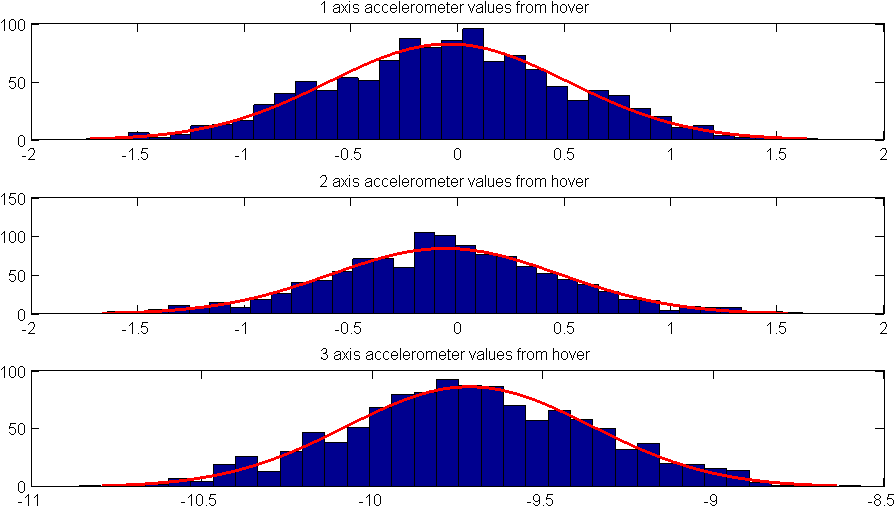
\includegraphics[width=\textwidth]{../rest_accel_hist.png}
\caption{Histogram of accelerometer readings during hover.}
\label{fig:accel_hist_hover}
\end{figure}

\subsection{Gyroscope}

Gyroscope measurements are evaluated in a similar fashion to the accelerometers; by comparing mean and standard deviation of errors at rest and in hovering flight. Typical bias should be well characterized by the measurements from rest. Position control mode is used for hovering flight, and it is thought that the mean angular rates should be zero for pitch and roll axes, and effectively constant for the yaw axis. The variance estimates are derived from hovering flight.

Tables \ref{tab:gyro}-\ref{tab:gyro_hover} show gyroscope measurement characteristics at rest and in hovering flight. The maximum standard deviation for any axis is approximately $0.12$ rad/s on any axis; conservatively, this is taken as the upper bound on all three axes, since there are no obvious typical differences in measurement variances between the three axes. Since much lower values are sometimes recorded, this value likely indicates a conservative upper bound. Mean gyro biases are frequently on the order of $0.001$ rad/s; a maximum bias of $0.015$ rad/s encompasses all the biases recorded in the tables.

Figs. \ref{fig:hover_gyro_hist} shows a histogram of the gyroscope measurements from the flight labelled ``Hover 2.'' This distribution is reasonably well-fit by a Gaussian distribution. In summary:

\begin{equation}
\sigma_{gX} = \sigma_{gY} = \sigma_{gZ} = 0.12 \ \mathrm{rad/s}
\end{equation}

\begin{figure}[tb!]
\centering
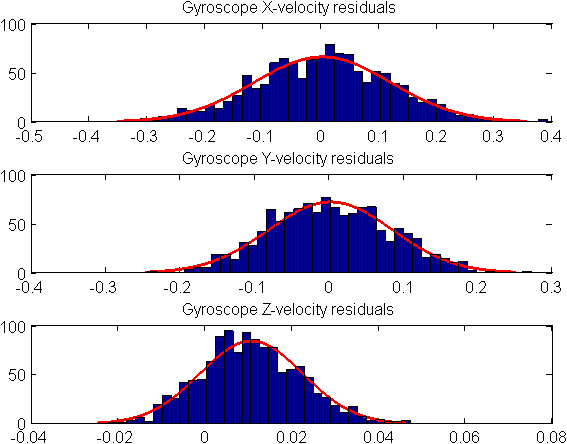
\includegraphics[scale=1]{../hover_gyro_hist.png}
\caption{Gyroscope measurement histograms from hovering flight.}
\label{fig:hover_gyro_hist}
\end{figure}

\begin{table}[tb!]
\centering
\begin{tabular}{c|c|c|c|c|c|c}
Data segment & $\mu_{gX}$ & $\mu_{gY}$ & $\mu_{gZ}$ & $\sigma_{gX}$ & $\sigma_{gY}$ & $\sigma_{gZ}$\\
Rest 1 & 0.0018 & -0.006 & -0.0043 & 0.017 & 0.017 &  0.014\\
Rest 2 & .0027 & -.0053 & -.0038 & 0.02 & 0.02 & 0.014\\
Rest 3 & -0.0023 & 0.00062 & -0.00087 & 0.03 & 0.027 & 0.025\\
Rest 4 & -0.0023 & -.00099 & -.0093 & 0.034 & 0.022 & 0.026\\
\end{tabular}
\caption{Summary of mean and standard deviation of gyroscope measurements with sensor at rest.}
\label{tab:gyro}
\end{table}

\begin{table}[tb!]
\centering
\begin{tabular}{c|c|c|c|c|c|c}
Data segment & $\mu_{gX}$ & $\mu_{gY}$ & $\mu_{gZ}$ & $\sigma_{gX}$ & $\sigma_{gY}$ & $\sigma_{gZ}$\\
Hover 1 & -2.2$\times 10^{-5}$ & -.0049 & 0.012 & 0.085 & 0.048 & 0.077\\
Hover 2 & 0.0023 & 0.0017 & 0.011 & 0.12 & 0.083 & 0.012 \\
\end{tabular}
\caption{Summary of mean and standard deviation of gyroscope measurements in hovering flight.}
\label{tab:gyro_hover}
\end{table}

\subsection{Ultrasonic rangefinder}

The ultrasonic rangefinder is one component of the optic flow sensor board. The rangefinder is characterized by comparing sensor returns against Optitrack position measurements. (This admits some error by neglecting consideration of attitude effects on the rangefinder outputs. Some bias between the center of mass defined in Optitrack and the location of the rangefinder is expected, and should be on the order of centimeters.) Fig. \ref{fig:movingflyingalt} shows typical rangefinder measurements compared to Optitrack data. The measurements match the Optitrack data well except for a notable number of outliers, which are clearly some sort of false returns. The rate of occurrence of these outliers is approximately 10\%, and is quantified in two tests.

Fig. \ref{fig:movingflyingalthist} shows a histogram of altitude errors once outliers are removed. More errors are concentrated near zero than the Gaussian distribution suggests, so this fit should be conservative. Table \ref{tab:altErrs} shows the mean and standard deviation of altitude measurement errors, ignoring outliers, as well as the fraction of samples that are outliers. It can be seen that the fraction of outliers may be quite high, and should be accounted for in data management. The bias is reasonably approximated as less than 5 centimeters typically (this figure includes uncertainty in the Optitrack-rangefinder relative offset). As a conservative bound, the 150\% of the maximum of the measured standard deviations is taken as the error bound:

\begin{equation}
\sigma_{alt} = 0.83 \ \mathrm{m}
\end{equation}

\begin{figure}[tb!]
\centering
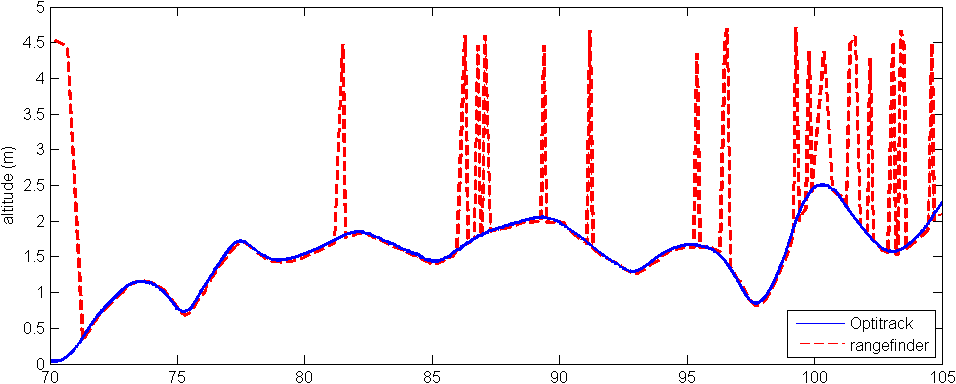
\includegraphics[width=\textwidth]{../moving_flying_alt.png}
\caption{Altitude measurements during flight.}
\label{fig:movingflyingalt}
\end{figure}

\begin{table}
\centering
\begin{tabular}{c|c|c|c}
Segment & Mean altitude error (m) & Error standard deviation (m)& Fraction of bad returns\\
1 & 0.035 & 0.055 & 0.20\\
2 & 0.026 & 0.031 & 0.085\\
\end{tabular}
\caption{Summary of in-flight errors from ultrasonic rangefinder.}
\label{tab:altErrs}
\end{table}

\begin{figure}[tb!]
\centering
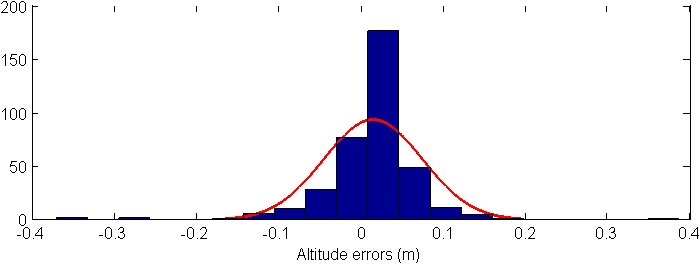
\includegraphics[width=\textwidth]{../moving_flying_alt_hist.png}
\caption{Histogram of ultrasonic rangefinder measurements after outliers are removed..}
\label{fig:movingflyingalthist}
\end{figure}

\subsection{Optic flow - ignore this and everything after, it's not finished}

%Fig. \ref{flowfft} shows the FFT of the optic flow measurements during hover. There are spikes around $10^{0.2},10^{0.35},10$ Hz that can be seen on multiple channels; the spikes are not very large and may not be significant. 

Table \ref{tab:flow} shows the mean and standard deviation of the optic flow measurements. The standard deviation for the compensated speeds are very large, on the order of tens of metres per second. 

Fig. \ref{fig:flowhist} shows histograms of each optic flow sensor measurement with a normal distribution best fit. Both the compensated x-velocity and the distance measurements have symmetric distributions with a higher concentration near the mean than a normal distribution. The compensated y-velocity appears to be right skewed, but the mean is still near zero. There may be additional bias that is not covered by the mean. The median value of the y-velocity is $-2$ m/s.

\begin{table}[tb!]
\begin{tabular}{c|c|c|c|c|c|c}
Flight segment & Mean CompX & Mean CompY & Mean distance & Std CompX & Std CompY & Std distance\\
Hover & 0.65 & 0.38 & -.014 & 13 & 24 & 0.29\\
\end{tabular}
\caption{Summary of mean and standard deviation of optic flow measurements.}
\label{tab:flow}
\end{table}

\begin{figure}[tb!]
\centering
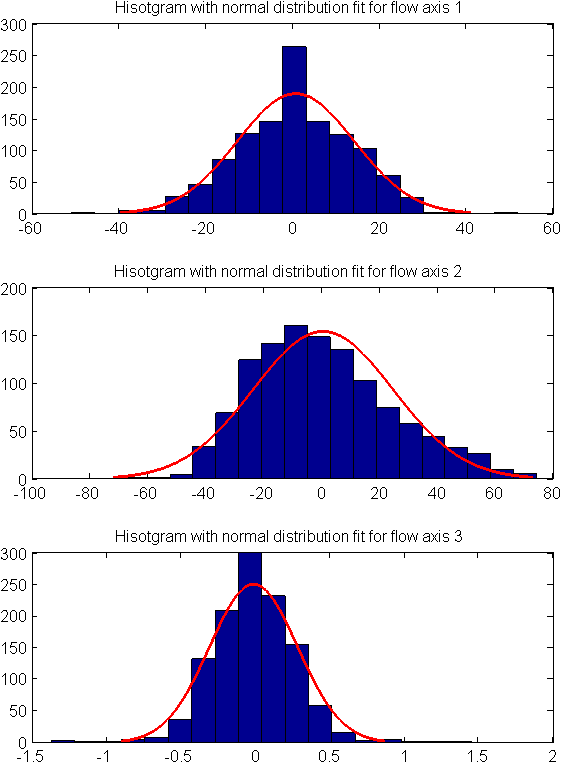
\includegraphics[scale=0.8]{../flowhist.png}
\caption{Histogram of optic flow measurements during hover.}
\label{fig:flowhist}
\end{figure}

\subsection{Moving cart optic flow}

Errors are computed by interpolating in the Optitrack data at the times velocities are recorded onboard the vehicle. 

\subsection{Flying in position control mode}

The vehicle is flown in position control mode at a constant altitude in several trials. To the extent possible, the body 1 and 2 axis velocities are excited individually. It should be noted that the optic flow sensor is aligned at 45\degree \ angle to the body axes. Truth values for the optic flow measurements are computed by rotating the Optitrack velocities into the body frame, then into the flow sensor frame. Time histories of Optitrack and optic flow measurements are shown in Fig. \ref{fig:movingflyingvelcomp}. Errors are computed only in the regions where optic flow data are plotted; in the intermediate regions, Optitrack position histories dropped out intermittently and truth velocities cannot be reliably computed.

\begin{figure}[tb!]
\centering
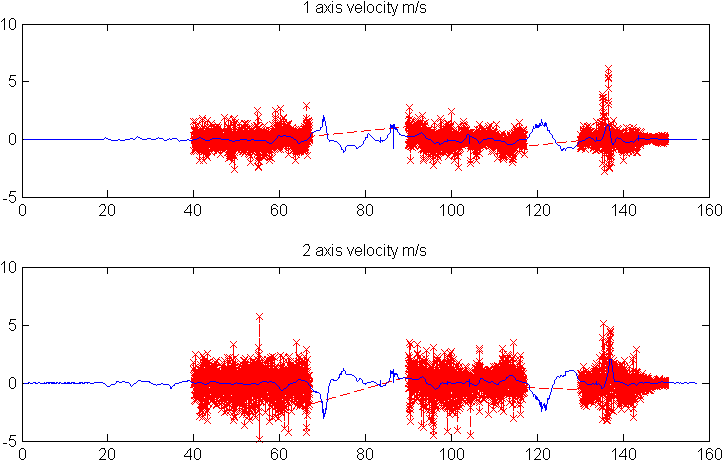
\includegraphics[scale=0.8]{../moving_flying_vel_comp.png}
\caption{Time histories of optic flow measurements and Optitrack truth data. Blue lines are the Optitrack data; red indicate optic flow measurements.}
\label{fig:movingflyingvelcomp}
\end{figure}

The mean residuals in the time segments considered are

\begin{eqnarray}
\bar{\epsilon}_x = .00091 \ \mathrm{m/s} \\
\bar{\epsilon}_y = .04 \ \mathrm{m/s}
\end{eqnarray}

The residual standard deviations are

\begin{eqnarray}
\sigma_x = 0.66 \ \mathrm{m/s} \\
\sigma_x = 1.1 \ \mathrm{m/s}
\end{eqnarray}

\begin{figure}[tb!]
\centering
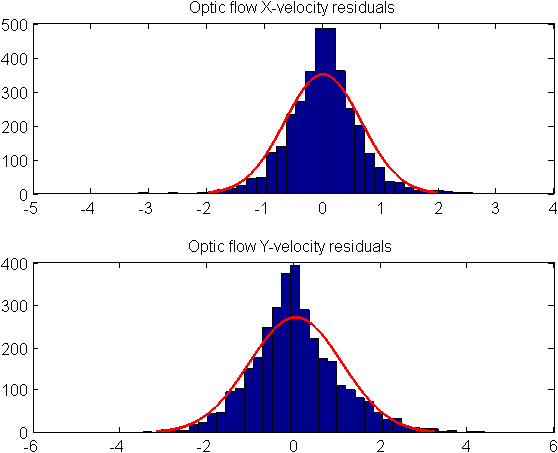
\includegraphics[scale=0.8]{../moving_flying_flow_hist.png}
\caption{Histograms of optic flow residuals during flight.}
\label{fig:movingflyingflowhist}
\end{figure}

Fig. \ref{fig:movingflyingflowhist} shows histograms of the computed errors. Results are reasonably Gaussian-like, and the fact that the data are concentrated more at the center than a true Gaussian indicates the standard deviations provide conservative bounds for errors.



%\printbibliography

\end{document}
